\chapter{Evaluation}
\label{ch:evaluation}


\section{Statistics}
\label{sec:statistics}

The statistical evaluation focused both at the extrinsic properties of the application and the development process itself (e.g. code volume, complexity, time spent on development), as well as the intrinsic functional properties of the core functionality that are reflected in the cost of \ac{CPU}-, network-usage and message latency.
Cost of rendering audio and video, as well as general user experience metrics were beyond the scope of the study, as these are highly specific to the task being implemented and are considered transient.

Computers used in the performance evaluation were end-user laptops with the following specifications: \emph{Computer A} is equipped with an 3.1GHz dual-core Intel Core i5 \ac{CPU}, 16GB of \ac{RAM} and a 500GB \ac{SSD}.
\emph{Computer B} is equipped with an Apple M1 Max \ac{CPU} with ten cores, 64GB of \ac{RAM} and a 1TB \ac{SSD}.
Both systems used the Google Chrome browser (version 121.0.6167.85), ran macOS 13.6.4 and connected to the network via 5GHz WiFi.
Both computers used the same \ac{NTP} server to synchronise clocks and the synchronisation was refreshed before each data sampling.

The \emph{latency measurements} were conducted for the data channels and over a consumer 50Mbit \ac{DSL} connection.
They were repeated at different times to account for variance in overall network service quality, and were also conducted over different international \ac{VPN} connections to simulate connection distances within and outside of Europe.
The measurements always used the \ac{BVH} data producer sending the message type for movement qualities alongside 29 key points at a rate of 25 messages per second.
Payload size was 453 bytes for each message, amounting to a required bandwidth of about 11.3 kilobytes per second for each motion capture data stream.
The audio streams were published alongside the data packets, but were not measured for latency.

The results for the latency analysis are shown in separate graphs for each computer containing the datasets for the local and remote messages on each device.

\begin{figure}[h]
\centering
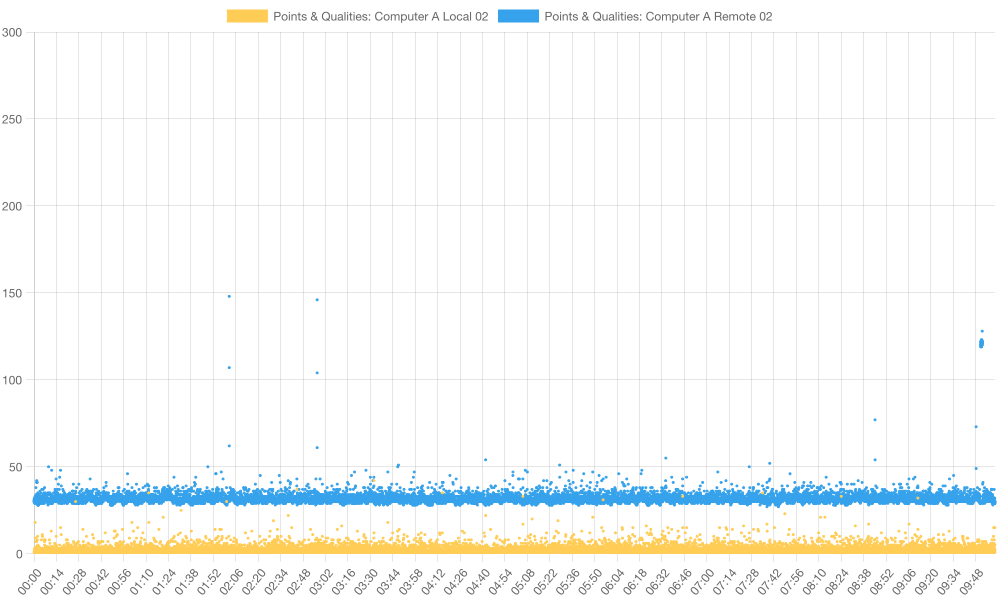
\includegraphics[scale=0.4]{04_Artefakte/01_Abbildungen/latency-computer-a-02}
\caption[Message latency on Computer A]{Computer A: Latency in milliseconds for local and remote messages\protect}
\label{fig:latencyComputerA}
\end{figure}

Results for computer A (\ref{fig:latencyComputerA}) show a median latency of 32ms for remote messages received over the WebRTC connection and 2ms for the connection from the local data producer to the browser.
Both values show a jitter at a variance of about 25ms for the remote connection and about 5ms for the local connection.

\begin{figure}[h]
\centering
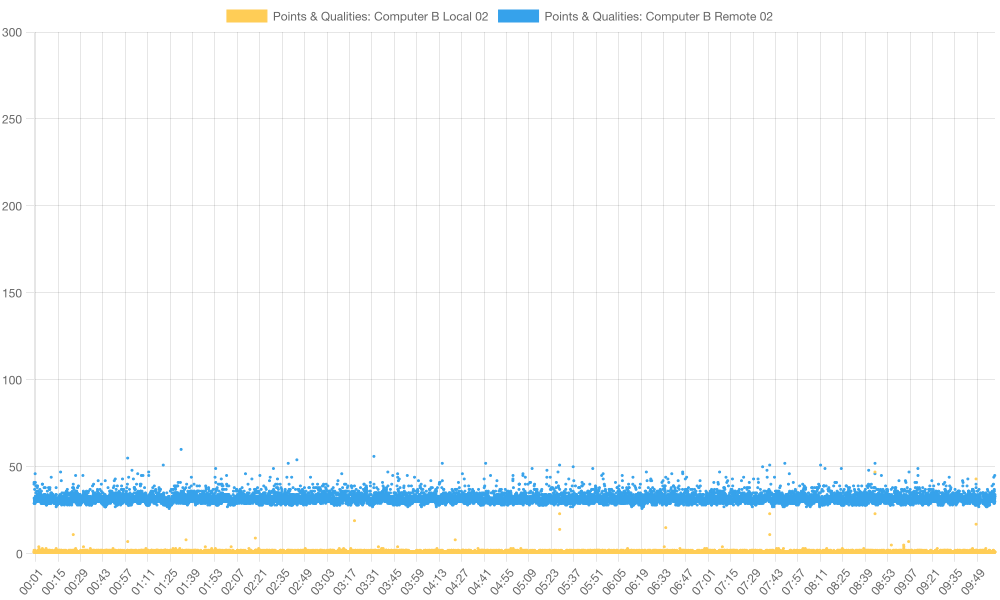
\includegraphics[scale=0.4]{04_Artefakte/01_Abbildungen/latency-computer-b-02}
\caption[Message latency on Computer B]{Computer B: Latency in milliseconds for local and remote messages\protect}
\label{fig:latencyComputerB}
\end{figure}

The results gathered on computer B (\ref{fig:latencyComputerB}) show a median latency of 31ms for the remote messages and 1ms for the local data producer connection.
Here, the jittering happens at a variance of about 7ms for the remote connection and about 1ms for the local connection.

The evaluation of time spent on the development work was based off the timesheets that were kept during the process. Only the time spent on the actual programming and infrastructure creation was tracked, as the research could not be properly separated from the work on the study itself. All recorded tasks were categorised by the language used (e.g. JavaScript vs. Python), the component worked on (e.g. \ac{UI} vs. \ac{API}) and the type of work (e.g. programming vs. administration).

In total, 96 work hours were spent on the creation of the reference implementation and its deployment on the test infrastructure. This would amount to 12 workdays, assuming eight hours for each day, which would be in line with §3 of the German law for labour time regulation, known as the \textquote{Arbeitszeitgesetz} (see \parencite{abzgPar3}).

\begin{figure}[h]
\centering
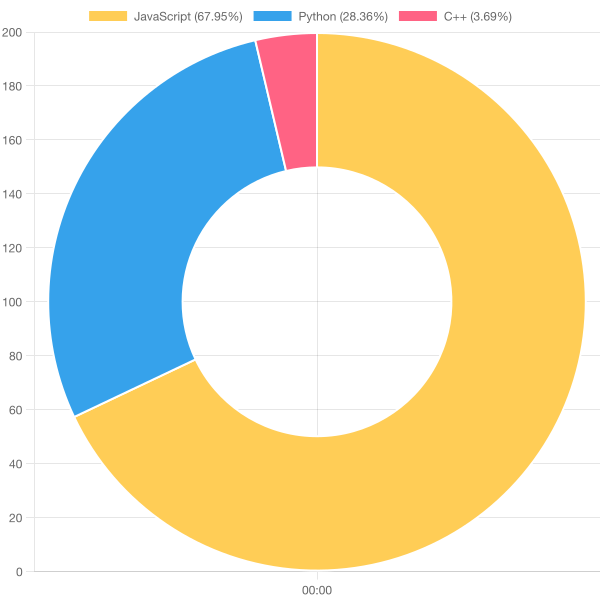
\includegraphics[scale=0.5]{04_Artefakte/01_Abbildungen/time-spent-on-languages}
\caption[Time spent on languages]{Time spent on various programming languages\protect}
\label{fig:timeSpentLanguages}
\end{figure}

The time spent on programming languages (\ref{fig:timeSpentLanguages}) shows a obvious lead for \ac{JS} being the most-used language, which would be rather obvious, given that it was chosen as the language for the \ac{UI} and the \ac{API}. However, Python still takes up almost a third of the work hours spent on programming. C and C++ required only a marginal amount of work with under 4\% of the time spent.

\begin{figure}[h]
\centering
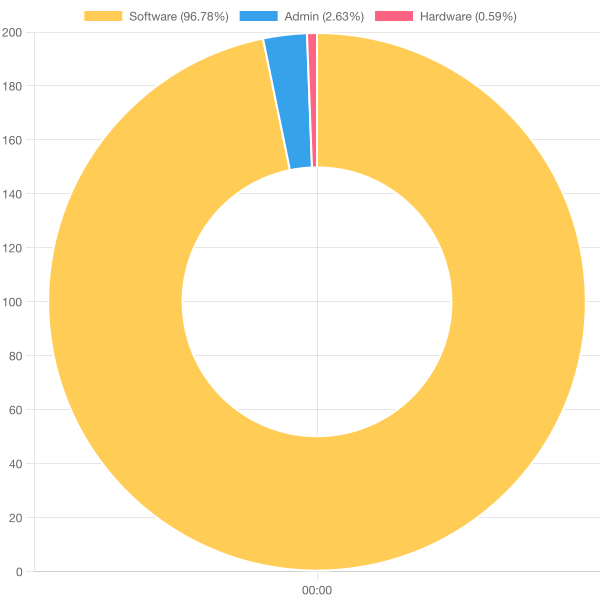
\includegraphics[scale=0.5]{04_Artefakte/01_Abbildungen/time-spent-on-types-of-work}
\caption[Time spent on areas of work]{Time spent on areas of work\protect}
\label{fig:timeSpentTypeOfWork}
\end{figure}

The distribution of time spent on software development versus setting up the infrastructure (administration) and constructing the head-tracker's hardware implementation (\ref{fig:timeSpentTypeOfWork}) clearly shows that almost all of the time (roughly 97\%) were spent on programming and the latter two factors were marginal in the effort needed to be put in.

\begin{figure}[h]
\centering
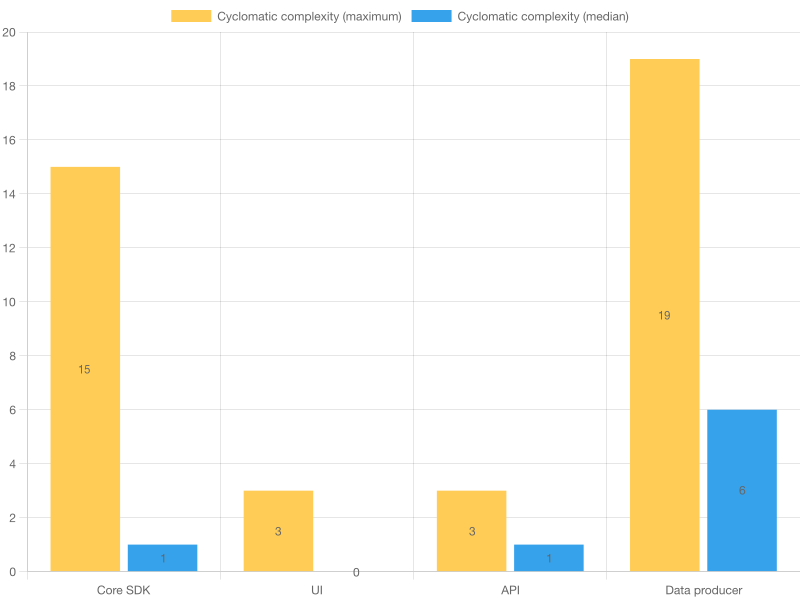
\includegraphics[scale=0.5]{04_Artefakte/01_Abbildungen/code-stats-complexity}
\caption[Cyclomatic complexity]{Cyclomatic complexity per component\protect}
\label{fig:cyclomaticComplexity}
\end{figure}

The cyclomatic complexity (\ref{fig:cyclomaticComplexity}) was only calculated for the core \ac{SDK}, the \ac{UI}, \ac{API} and the general data producer. The Arduino code does not use any branching and the C++ code for the Captury producer was deemed a workaround since it should be integrated in the Python structure for proper use. The maximum complexity shows a large overhead exceeding the recommended thresholds (see \autoref{ch:methodology}) on behalf of the core \ac{SDK} with 15 and for the data producer with 19, although the median values show a distinct concentration of complexity with the data producer (6 versus 1 for the \ac{SDK}). This shows that the massive complexity value of 15 rather is an outlier for the \ac{SDK}, but seems more intrinsic to the data producer's structure. The \ac{UI} and \ac{API} however, show a very low overall complexity, which was the desired outcome to keep these parts more hackable and easy to grasp.

\begin{figure}[h]
\centering
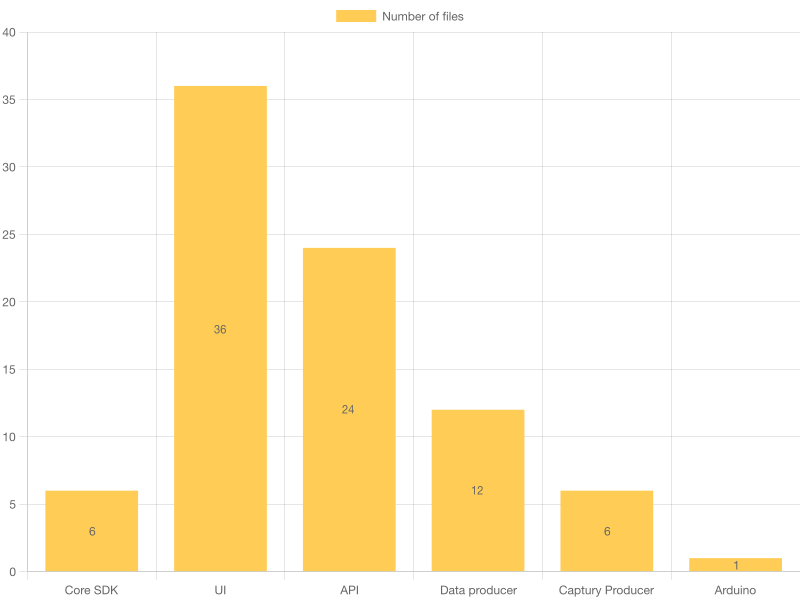
\includegraphics[scale=0.5]{04_Artefakte/01_Abbildungen/code-stats-filecount}
\caption[File count]{Number of source files per application component\protect}
\label{fig:fileCount}
\end{figure}

In terms of weight measured by the number of files (\ref{fig:fileCount}), the most code files were produced for the \ac{UI} and the \ac{API}, which aligns with the distribution of functionality according to the concept. In general, it shows a relatively moderate weight for the entire application with 36 files created for the \ac{UI} and an average of roughly 14 files across all components.

\begin{figure}[h]
\centering
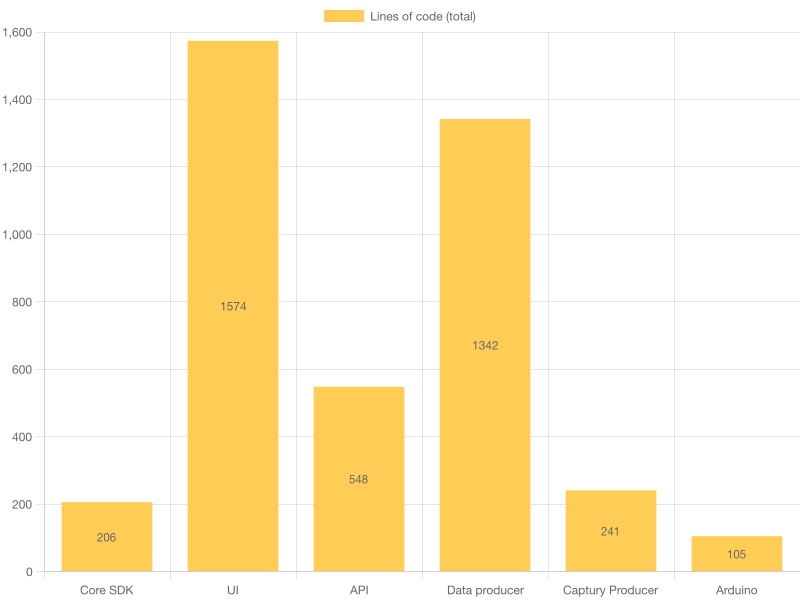
\includegraphics[scale=0.5]{04_Artefakte/01_Abbildungen/code-stats-loc-total}
\caption[Lines of code (total)]{Total lines of code per application component\protect}
\label{fig:linesOfCodeTotal}
\end{figure}

The distribution of weight in regard to the total lines of code without comments produced for each component (\ref{fig:linesOfCodeTotal}) aligns with the number of files for the \ac{UI}, but shows a large overhead for the data producer with almost as many lines of code distributed among a third of the number of files.

\begin{figure}[h]
\centering
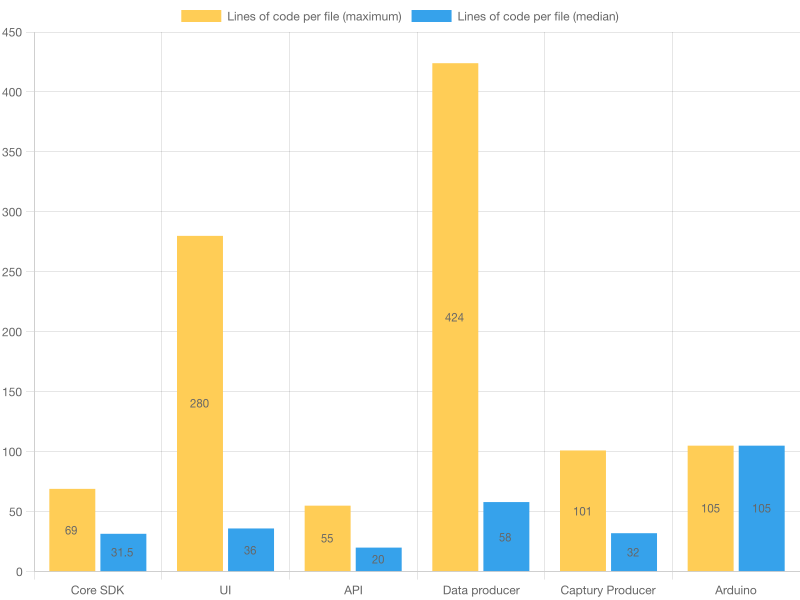
\includegraphics[scale=0.5]{04_Artefakte/01_Abbildungen/code-stats-loc}
\caption[Lines of code]{Maximum and median number of lines of code per application component\protect}
\label{fig:linesOfCode}
\end{figure}

Median and maximum amounts of lines of code across files for each component (\ref{fig:linesOfCode}) show a moderate distribution with the median at about half or a third of the maxium value and below the recommended thresholds (see \autoref{ch:methodology}). Again, the only exception to this is the data producer that, while showing a normal median, shows a maximum of 424 lines of code.

\section{Critical reflection}
\label{sec:critical-reflection}

The development process was carried out in two main timeframes (X and Y) and followed the guiding principles decided in the concept.
It was a mostly pleasant experience with the selected frameworks delivering on their promised functionality and ease of use.
The initial setup was extremely quick due to the ease of setup of the WebRTC server and the quick generation of boilerplate code for the \ac{API} and the \ac{UI}.
However, the web audio standard implementation leaves a lot to desire, especially the support for spatial audio in the browser.
Currently, there is no built-in way to load custom \ac{HRTF} data, which should drastically improve the accuracy of spatial positioning for sound.
There are approaches using a custom build of the Chromium browser~\parencite{chromiumCustomHrtf} or a custom audio node~\parencite{customHrtfAudioNode} which unfortunately does not work with the \ac{SOFA} file format, so it is generally rather disappointing not seeing this thoroughly implemented in the general standard \ac{API}.

The initial setup for the data producers was also relatively quick, due to the large number of examples for the DepthAI \ac{SDK} and the clarity and hands-on approach to the main Python documentation.
The only thing lacking here, was a straightforward way to manage dependencies, as there were different results for the same dependencies being installed via PIP or Conda.

